%\documentclass[11pt]{article}
\documentclass[11pt]{amsart}
\usepackage{graphicx,xspace}
\usepackage{fullpage}
\usepackage{hyperref}
\usepackage{amsmath}
\usepackage{amsfonts}
\usepackage{verbatim}
\newenvironment{definition}[1][Definition]{\begin{trivlist}
\item[\hskip \labelsep {\bfseries #1}]}{\end{trivlist}}
\newenvironment{example}[1][Example]{\begin{trivlist}
\item[\hskip \labelsep {\bfseries #1}]}{\end{trivlist}}
\title{ADAM: Analysis of Discrete Models of Biological
Systems Using Computer Algebra}
\author{Franziska Hinkelmann$^{a,b}$,
Madison Brandon$^{c,*}$,
Bonny Guang$^{d,*}$,
Rustin McNeill$^{e,*}$, \\
Grigoriy Blekherman$^{a}$,
Alan Veliz-Cuba$^{a,b}$,
Reinhard Laubenbacher$^{a,b}$}
\begin{document}
\maketitle
{\footnotesize
            \centerline{$^a$Virginia Bioinformatics Institute, Blacksburg, VA 24061-0123, USA}
}
{\footnotesize
            \centerline{$^b$Department of Mathematics,
             Virginia Polytechnic Institute and State University, Blacksburg, VA 24061-0123, USA}
}
{\footnotesize
            \centerline{$^c$University of Tennessee - Knoxville, Knoxville, TN 37996-2513, USA}
}
{\footnotesize
            \centerline{$^d$Harvey Mudd College, Claremont, CA 91711-5901, USA}
}
{\footnotesize
            \centerline{$^e$University of North Carolina - Greensboro, Greensboro, NC 27402-6170, USA}
}
{\footnotesize
            \centerline{$^*$These authors contributed equally}
}
%%%%%%%%%%%%%%%%%%%%%%%%%%%%%%%%%%%%%%%%%%%%%%%%%%%%%%%%%%%%%%%%%%
\begin{abstract}
{\bf Motivation:} Many biological systems are modeled qualitatively with discrete models, such as
probabilistic Boolean networks, logical models, bounded Petri nets, and agent-based models.
Simulation is a common practice for analyzing discrete models, but many systems are far too large
to capture all the relevant dynamical features through simulation alone. \\
{\bf Results:} We convert discrete models into algebraic models
and apply tools from computational algebra to analyze their dynamics.
The key feature of biological systems that is exploited by our algorithms is their sparsity: while the number of nodes in a
biological network may be quite large, each node is affected only by a small number of other nodes. In our experience with models arising in systems biology and random models, this structure leads to fast
computations when using algebraic models, and thus efficient analysis.\\
{\bf Availability:} All algorithms and methods are available in our package Analysis of Dynamic
Algebraic Models (ADAM), a user friendly web-interface
that allows for fast analysis of large models, without requiring understanding of the underlying mathematics or any software installation. ADAM is available as a web tool, so it runs platform independent on all systems.\\
{\bf Contact:} \href{mailto:reinhard@vbi.vt.edu}{reinhard@vbi.vt.edu}\\
\end{abstract}
%%%%%%%%%%%%%%%%%%%%%%%%%%%%%%%%%%%%%%%%%%%%%%%%%%%%%%%%%%%%%%%%%%
\section{Introduction}
% Different discrete models and lack of analysis tools
Mathematical modeling is a crucial tool in understanding the dynamic behavior of complex
biological systems. Discrete models are now widely used for this purpose.  Model types include
(probabilistic) Boolean networks, logical networks, Petri nets, cellular
automata, and agent-based (individual-based) models, to name the most commonly found ones \cite{Steggles, heiner-petri, shmulevich, Chaouiya, cell-automata, springer_book}.



\begin{comment}Simulation is especially inefficient for non-deterministic
systems, since simulations must be run many times to obtain meaningful
probability estimates.
\end{comment}

%include a review of existing software, ginsim, boolnet, DDLab, Shmulevich, PetriNet (Snoopy) %etc and their capabilities regarding
%large models.
There are several existing software packages for analysis of discrete models. Each package has been developed to suit the needs of a particular community, and each package is designed to analyze a single model type. We briefly discuss some of their features below.


{\it GINsim} (Gene Interaction Network simulation) is a package designed for analysis of gene regulatory networks \cite{GINsim}. As input, it accepts logical models. Logical models are an extension to Boolean models; they consist of similar switch-like rules, but allow for a finer discretization than two states per variable, e.g., low, medium, and high. The temporal evolution of a logical model is non-deterministic for a given initial configuration, as the variables are updated randomly in an asynchronous fashion. In addition to being a tool for modeling and simulation, GINsim supports algorithms facilitating the representation as decision diagrams to determine steady states and oscillatory behavior \cite{Chaouiya}. For synchronous updates, analysis of limit cycles is only possible via simulation, meaning that an
initial configuration of the system is iterated a prescribed number of times, or until a
steady state is found. Since the number of initial configurations grows exponentially in the number of variables, simulation
will not provide a complete picture of dynamical behavior for large models. Thus, analysis by simulation is limited by the network size.   



{\it BoolNet R package} has methods for inference and analysis of synchronous, asynchronous, and probabilistic Boolean networks \cite{boolnet}. Steady state analysis is done via exhaustive enumeration of the state space, heuristic search, random walk, or Markov Chain analysis \cite{shmulevich}. Again, analysis is limited by model size (exhaustive enumeration or Markov Chain analysis) or restricted to heuristic methods, which might fail to detect some key dynamic features.


{\it Snoopy} is a unifying Petri net framework, containing a family of Petri net modeling tools and algorithms \cite{Snoopy}. Snoopy provides simulation and built-in animation. Analysis of Petri nets can be done, e.g., with the tool Charlie \cite{Charlie}. Charlie can identify structural properties and has algorithms for invariant based or reachability graph based analysis. Analysis for Petri nets is usually based on a given initial state and does not provide a complete picture of possible dynamics for other initial states.

{\it DDLab} is an interactive graphics software for discrete models, including cellular automata, Boolean and multi-valued networks. As it is mainly a visualization tool, analysis is based on exhaustive enumeration of the state space.



In summary, except for GINsim for asynchronous logical models, these tools provide a complete analysis of the dynamical behavior only if an exhaustive enumeration of the state space is computationally feasible. 




Here, we present the online software package ADAM, Analysis of Dynamic Algebraic Models \cite{ADAM}, an analysis tool to study the dynamics of a wide range of discrete models. ADAM is the successor to DVD, Discrete Visualizer of Dynamics \cite{DVD}, a tool to visualize the temporal evolution of small polynomial dynamical systems. All of the different types of discrete models mentioned above can be
converted into the unified framework of polynomial dynamical systems
\cite{Alan:Bioinf2010, Hinkelmann:2010}. This allows us to apply tools from
computational commutative algebra to analyze their dynamics more efficiently than by simulation and without using heuristic methods. In addition, using a unifying framework for several model types
allows for an effective comparison of heterogeneous models, such as a Boolean network model and an agent-based model.
For community integration to the biological sciences, ADAM contains a model repository of  previously published models available in ADAM specific format. This allows new users to quickly familiarize themselves with ADAM and to validate and experiment with existing models.
\begin{comment}General features of ADAM are discussed briefly, and new features are explained more in detail. \end{comment}
In the following, we discuss general features of ADAM briefly and explain new features in more detail.

%%%%%%%%%%%%%%%%%%
\section{General Features}
ADAM automatically converts discrete models into polynomial dynamical
systems, that is time and state discrete dynamical systems described by polynomials over a finite field (see Appendix \ref{pds} for definition and example),
%*************************************
%
%need a definition here rather than asking the reader to go to the appendix. This is a central
%concept in the paper. Greg and I would rather have the definition in the appendix, because %there’s no other formulas anywhere in the paper.
%
%*************************************
and then analyzes their dynamics by using various computational algebra techniques. Even for large systems, ADAM
computes key dynamic features, such as steady states, in a matter of seconds.
ADAM is available online, free of charge. It is platform
independent and does not require installation of any software or computer
algebra tool.
%% different input types
ADAM can analyze discrete models. It supports the following {\bf inputs}.
\begin{itemize}
\item Logical models generated with GINsim \cite{GINsim}
\item Petri nets generated with Snoopy \cite{Snoopy}
\item polynomial dynamical systems
\item Boolean networks
\item probabilistic polynomial dynamical systems \cite{shmulevich}.
\end{itemize}
ADAM’s purpose is analysis of the dynamic features of a model. ADAM can find stable attractors of dynamical systems. These are either steady states, i.e., time-invariant states,
or limit cycles, i.e., a collection of states between which the systems oscillates. ADAM is capable of identifying steady states and limit cycles of length up to a user-specified length $m$. The process of finding long limit cycles is quite slow for large models, however, in biological models limit cycles are likely to be short, so that $m$ can be chosen to be small in general.

The temporal evolution of the model can be visualized by the {\it phase space}, a graph of all possible states and their transitions. For small enough models, ADAM generates a graph of the complete phase space. Independent of network size, ADAM generates a {\it wiring diagram}. Wiring diagrams, also known as dependency graphs, show the static relationship between the variables. All edges in ADAM’s wiring diagrams are functional edges, that is for some configuration of the system, a change in the input variable causes a change in the output variable (see Appendix \ref{sec:func} for more details). This means that ADAM determines all non-functional edges, which is oftentimes of interest.
ADAM can also be used to study evolution of user-specified initial states. The evolution of a single state can be determined by computing the trajectory initiating from this state and evaluating it until an attractor is reached.

All of these features can be computed assuming synchronous update, or an asynchronous update schedule specified by the user. Note that the steady states are the same independent of the update schedule. This is due to the fact that updating any variable at a steady state does not change its value. Thus, it is irrelevant whether one updates sequentially or simultaneously.  

%***********************************
%
%need a reference or an explanation here
%is this ok?
%
%**********************************

For probabilistic networks, i.e., models in which each variable has several choices of local update rules, ADAM can generate a graph of all possible updates. This means that states in the phase space have out degree $\geq 1$, since there are several transitions possible. ADAM can find all true  steady states, i.e., states where any combination of possible update rules transitions to the same state. For further information of probabilistic networks, see \cite{shmulevich}.

For Boolean networks, ADAM calculates all functional circuits (see Appendix \ref{sec:func}). For a certain class of Boolean networks, namely conjunctive/disjunctive networks, ADAM computes a complete description of the phase space (see Appendix \ref{sec:conj}).
In summary, ADAM can generate the following {\bf outputs}.
\begin{itemize}
\item a graph of wiring diagram
\item steady states (for deterministic and probabilistic systems)
\item limit cycles of specified length $m$
\item trajectories originating from a given initial state until a stable
attractor is found
\item dynamics for synchronous or asynchronous updates
\item functional circuits for Boolean networks
\item a complete description of the phase space for conjunctive/disjunctive
networks.
\end{itemize}
%%%%%%%%%%%%%%%%%%%%%%%%%%%%%%%%%%%%%%%%%%%%%%%%%%%%%%%%%%%%%%%%%%
\section{Methods}
Logical models, Petri nets, and Boolean networks are automatically converted
into the corresponding polynomial dynamical system as described in
\cite{Alan:Bioinf2010}, so that algorithms from computational
algebra can be used to analyze the dynamics.

We developed and implemented several different algorithms that allow one to analyze
important features of algebraic models when they are too large for exhaustive simulation.
Most algorithms rely on Gr\"obner basis calculations to find key dynamic
features. Gr\"obner basis calculation is for polynomial systems what
Gauss-Jordan elimination is for linear systems: a structured way to transform
the original system to triangular shape without changing its solution space.
The triangular shape of the resulting systems allows for stepwise retrieval of the solutions of the system. For a more in depth discussion of Gr\"obner bases, see for example \cite{IVA}.

%**********************************************
%
%the reader is likely to encounter this term for the first time, so we need a reference or
%explanation here. - we moved up the description from below and cite iva
%
%
%*******************************************

Since the polynomials in the algebraic
models originate from biological systems, we can exploit their structural
features to secure very fast Gr\"obner basis computations.
%explain that everything is a polynomial and how equations relate to dynamics
The key idea behind our algorithms is that discrete models have finitely many states and computations
can be performed over a finite field \cite{Alan:Bioinf2010,
Hinkelmann:2010}, that is, a finite number system analogous to the Boolean field with two elements.
Since any function over a finite field is a polynomial
\cite{Lidl:1997} we convert discrete models into polynomial dynamical systems
and use commutative algebra algorithms. More specifically, the problem of finding steady states and limit cycles
can now be reformulated as solving a system of polynomial equations (see the Appendix for details).

% Sparse systems
The efficiency of the Gr\"obner basis calculations is largely dependent on the
assumption that most discrete models arising from biological systems are
sparse, meaning that every variable is only affected by a small subset of the
total variables in the system. It has been suggested, that in robust gene
regulatory networks genes are regulated by only a handful of regulators
\cite{Leclerc:2008}. Thus, the polynomial dynamical systems representing such biological networks are
sparse, i.e., each function depends only on a small subset of the model variables.

% heuristic explanation for why we think the GB algorithm is fast on
% sparse systems..
In the worst case, computing Gr\"obner bases for a set of polynomials has
complexity doubly exponential in the number of solutions to the system.
However, in practice, Gr\"{o}bner bases are computable in a reasonable time, and, from our experience,
for the sparse systems over a finite field that are common in discrete
biological models, it is actually quite fast.
Based on benchmarking tests for
25 logical models of biological systems \cite{GINsimRepo}
and randomly generated systems,
the computations for models arising in systems biology are very fast, and finish on the scale of
seconds.

\section{Application} \label{benchmarks}
% Example application
We demonstrate the strength of ADAM on a well-understood model of the expression
pattern of the segment polarity genes in Drosophila melanogaster. Albert and Othmer developed a model for embryonic pattern formation in the fruit fly Drosophila melanogaster \cite{AO}. Their Boolean
model consists of 60 variables, resulting in a phase
space with more than $10^{18}$ states. They analyze the model for steady states by setting up a system of Boolean equations and manually solving it. They also analyze the temporal evolution of a specific initial state corresponding to the wild type expression pattern by repeatedly applying the Boolean update rules until the steady state is found. The update schedule of the model is synchronous  with the exception of activation of SMO and the binding of PTC to HH (activation of PH), which are assumed to happen instantaneously. This can be accounted for by substituting the equations for SMO and PH into the update rules for other genes and proteins, rather than using SMO and PH themselves.

To analyze the model with ADAM, we rename the variables in the Boolean rules given in \cite{AO} to $x_i$. Then we can use ADAM to analyze the model: the model type is {\it PDS}, the number of states in a Boolean model is $2$, i.e., present or absent. One can pick {\it Boolean}, and enter the Boolean rules in the text-area or upload a text file with the Boolean rules. Alternatively, one can first convert the Boolean rules to polynomials over $\mathbb F_2$, and enter the polynomials with the choice {\it Polynomial}.
The file with a complete description for the model can be accessed at \cite{DrosophilaModel}. The rules in the model file are specified in {\it Polynomial} form. Once the polynomials are uploaded, we need to choose the {\it Analysis} type. The model with $60$ variables is too complex for simulation, and we choose {\it Algorithm}. This means that instead of exhaustive enumeration of the state space, analysis of the dynamics is done via computer algebra by solving systems of equations.
In {\it Options}, we set {\it Limit cycle length} to $1$ since we are looking for steady states, i.e., time-invariant states.
We chose {\it synchronous} as updating scheme. Once these choices have been made,
we obtain the steady states by clicking {\it Analyze}.
ADAM returns a link to the {\it wiring diagram} or dependency graph, which captures the static relations between the different variables. Below, ADAM returns the number of steady states and the steady states themselves.
Each row in the table corresponds to a stable attractor. Attractors are written as binary strings, e.g.,
\begin{align*}
(&0 0 0 1 1 1 1 0 0 0 1 0 0 0 0\\
&0 0 0 0 0 0 0 1 1 1 1 1 1 1 0\\
&1 0 0 0 0 0 0 0 1 0 0 1 1 0 1\\
&1 1 1 0 0 0 0 1 1 1 1 1 1 1 0).
\end{align*}
This corresponds to the configuration of the system with the first 8 proteins and genes absent, the next one present, the next two absent, etc. In fact, this is exactly the steady state obtained in \cite[Figure 4(b)]{AO} when starting the system with an initial state representing the experimental observations of stage 8 embryos. Note that we include variables for SLP, which are not shown in \cite[Figure 4(b)]{AO} as they are fixed to be $0011$ throughout the paper. The output is shown in Fig \ref{fig:alg}.
\begin{figure}[htb]
\centering
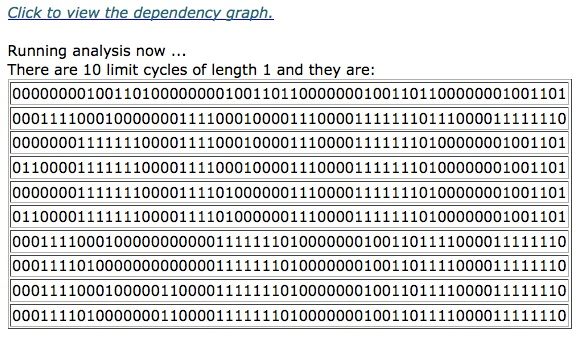
\includegraphics[width=0.95\textwidth]{DroAlgOutput.jpg}
\caption{ADAM: Analysis of steady states of Drosophila model}
\label{fig:alg}
\end{figure}


ADAM can also generate trajectories for a given initial state. For example, we
can pick the initial state that was used in \cite[Figure 4(a)]{AO}. Again, we
enter {\it PDS} with $2$ as the number of states and upload the polynomials
describing the model. Instead of {\it Algorithms}, we now choose {\it
Simulation}. Since we are not interested in the number of steady states or the
complete phase space, but in a single trajectory originating from a specific
initial state,  we choose {\it One trajectory starting at an initial state} as the simulation option. As
initial state we enter the one corresponding to \cite[Figure 4(a)]{AO},
\begin{align*}
(&0 0 0 1 0 1 0 0 0 0 0 0 0 0 0\\
&0 0 0 0 0 0 0 1 0 0 0 1 0 0 0\\
&1 0 0 0 0 0 0 1 0 0 0 1 0 0 0\\
&1 1 0 0 0 0 0 1 0 0 0 1 0 0 0).
\end{align*}
By clicking {\it Analyze}, we obtain the temporal evolution of this particular
state until it reaches a steady state. As predicted in \cite{AO}, the
steady state is the steady state from the previous paragraph, see Fig.
\ref{fig:traj}.
\begin{figure}[htb]
\centering
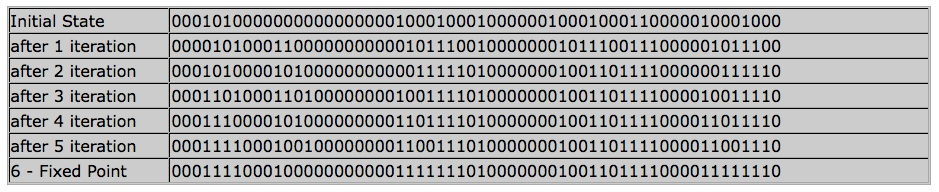
\includegraphics[width=0.95\textwidth]{DroTraj.jpg}
\caption{ADAM: Trajectory of Drosophila model}
\label{fig:traj}
\end{figure}
To summarize, ADAM correctly identifies the steady states
in less than one second. All steady states have been determined previously in \cite{AO} by labor-intensive manual investigation of the system. In \cite{AO}, the model is formulated as a set of Boolean rules. In order to determine the steady states, the system of Boolean expressions was solved manually.
In addition, we used ADAM to verify that are there no limit
cycles of length two or three. The model has not been analyzed previously for
limit cycles. The absence of two- and three cycles strengthens confidence in
the model, since oscillatory behavior has not been observed experimentally.
The model file in ADAM format can be accessed at \cite{DrosophilaModel}.
\subsection{Benchmark Calculations}
We analyzed logical models
available in the GINsim model repository \cite{GINsimRepo} as of August 2010. The
repository consists of models in GINsim XML format previously published in
peer-reviewed journals. We converted all but two models into polynomial
dynamics systems. For these 27 models we computed the steady states. Almost all
calculations finished in less than a second. The two largest networks,
consisting of over $10^{30}$ states, took approximately 20 minutes each, see
Figure \ref{fig:chart}.
In addition to the published models in \cite{GINsimRepo}, we analyzed
randomly generated networks
that have the same sparse structure that we
expect from biological systems. We tested a total of 50 networks with
50-100 nodes ($10^{15} - 10^{30}$ states) and up to two inputs per variable. The
steady state calculations took less than half a second for each network on
a 2.7 GHz computer.
\begin{figure}[htb]
\centering
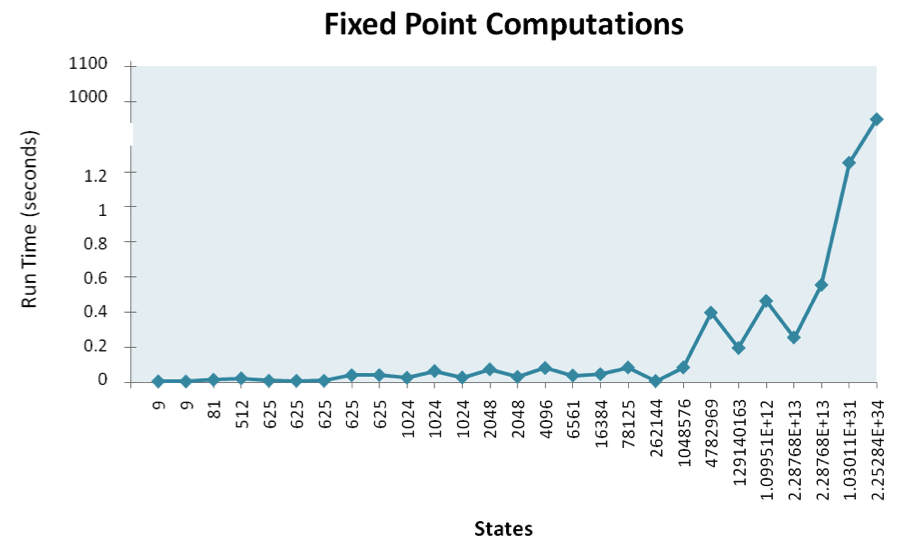
\includegraphics[width=0.7\textwidth]{GINSimChart.png}
\caption{Runtime of steady state calculations of several logical models from
\cite{GINsimRepo}. Executed on a 2.7 GHz computer.}
\label{fig:chart}
\end{figure}

%%%%%%%%%%%%%%%%%%%%%%%%%%%%%%%%%%%%%%%%%%%%%%%%%%%%%%%%%%%%%%%%%%
\section{Architecture}
ADAM is available as an online-tool, with no need for the user to install any software. ADAM's user interface is implemented in HTML. We use JavaScript to generate a dynamic website that adapts as the user makes various choices. This simplifies the process of entering a model. For example, after defining the model type, i.e., Polynomial Dynamical System, Probabilistic Network, Petri net, and Logical Model the next line changes to the number of states, $k$-bound, or nothing, appropriately. Input can be entered directly into the text-area on the form, or uploaded as a text document.

All mathematical algorithms are programmed in Macaulay2 \cite{M2}. Macaulay2 is a powerful computer algebra system. The routines for which fast execution is crucial are implemented in C/C++ as part of the Macaulay2 core. Logical Models and Petri nets in XML format are parsed using Ruby's XmlSimple library. The interplay between HTML and Macaulay2 is also programmed in Ruby.

Output graphs are generated with Graphviz's {\it dot} command. When {\it Simulation} is chosen as analysis method, Graphviz's {\it ccomps - connected components filter for graphs} is used to count the connected components. A Perl script directs the execution of the Graphviz commands.
%%%%%%%%%%%%%%%%%%%%%%%%%%%%%%%%%%%%%%%%%%%%%%%%%%%%%%%%%%%%%%%%%%
\section{Model Repository}
\begin{comment}In order to be compatible with other modeling software, ADAM can analyze logical models in GINsim XML format \cite{GINsim}, as well as Petri nets generated with Snoopy \cite{Snoopy}, also as XML model file. This allows modelers from the Logical models or Petri net community to benefit from ADAM's powerful analysis methods. Files in these XML formats can be directly uploaded to the website and then simulated or analyzed as polynomial dynamical systems. Conversion happens automatically, as a result, the user is given a list of variable names (as specified in the XML file), and the corresponding $x_i$ used in the polynomial dynamical system, so that the output can easily be interpreted.

ADAM generates several graphs. Users can choose between several output formats (gif, jpeg, pdf, and ps), so that the generated pictures can be used without further changes within several different text editing packages.
\end{comment}
A model repository is part of the ADAM website. The repository consists of a collection of several previously published models in ADAM format. The models are extracted from publications, and rewritten in ADAM specific format, i.e., all variables are renamed to $x_i$ and the update rules from the original publication are reformulated as Boolean rules or polynomials. A central repository with models in a unified framework allows for quick verification and experimentation with published models. By changing parameters or initial states the users can gain a better understanding of the models.

New users can also use the repository to quickly familiarize themselves with the main functionalities of ADAM. In addition to the model itself, the database entries contain a short summary of the biological system and relevant graphs, together with an analysis of dynamic features determined by ADAM and their biological explanation. The repository is a work in progress by researchers from several institutions generating more entries for the repository.  We invite all interested researchers to submit their models.


Because of their intuitive nature, discrete models are an excellent introduction to mathematical modeling for students of the life sciences. ADAM's model repository is a great starting point to familiarize students with the abstraction of discrete models such as Boolean networks.
%%%%%%%%%%%%%%%%%%%%%%%%%%%%%%%%%%%%%%%%%%%%%%%%%%%%%%%%%%%%%%%%%%
\section{Conclusion}
Discrete modeling techniques are a useful tool for analyzing biological
systems. Upon translating a discrete model, such as logical networks,
Petri nets, or agent-based models into an algebraic model, rich mathematical
theory becomes available. This opens up possibilities for analysis of dynamics with methods other than
simulation, which is limited due to combinatorial explosion. After extensive experimentation with both discrete models arising in systems biology and randomly generated networks, we found that our algorithms
are fast for sparse systems, a structure maintained by most biological
systems. All algorithms have been included in the software package ADAM\cite{ADAM},
which is user-friendly and available as a free web service.
ADAM is highly suitable to be used in a classroom as a first
introduction to discrete models as it does not require the students to run
anything else but a web browser.

%need to compare and contrast ADAM with the other available packages reviewed earlier.
There are  several software tools for discrete models, all of them specializing in a single discrete model type.
{\it GINsim}, a tool for modeling and simulation of logical models can quickly identify steady states \cite{GINsim}, but it has no other means than simulation to identify limit cycles for synchronous networks. {\it BoolNet R package}, a package for inference and analysis of synchronous, asynchronous, and probabilistic Boolean networks, does a steady state analysis by exhaustive enumeration of the state space or heuristic methods \cite{boolnet}. Analysis is limited by model size (exhaustive enumeration or Markov Chain analysis ) or restricted to heuristic methods, which might fail to detect some key dynamic features.
{\it Snoopy} and {\it Charlie}, software tools for Petri nets, base all their analysis methods on a given initial marking and do not contain any methods to analyze the complete possible phase space, when no marking is given. {\it DDLab}, an interactive graphics software for cellular automata, Boolean and multi-valued networks, does not provide analysis methods other than through visualization. Simulation or visualization are always limited by model size or restricted to a small part of the state space.

For all these types of discrete models, ADAM provides methods to analyze the key dynamic features, such as steady states and limit cycles, for large-scale models. ADAM unifies different modeling types by providing analysis methods for all of them and thus can be used by a larger community.

We hope to expand ADAM to a more comprehensive Discrete Toolkit which incorporates more
analytical methods, better visualization, and automatic conversion for more model types.
We also hope to analyze controlled algebraic models and expand theory to stochastic systems.


%%%%%%%%%%%%%%%%%%%%%%%%%%%%%%%%%%%%%%%%%%%%%%%%%%%%%%%%%%%%%%%%%%
\appendix
\section{Mathematical Background}
\subsection{Polynomial Dynamical Systems}
To be self-contained, we briefly explain polynomial dynamical systems and their key features.

\subsubsection{Polynomial Dynamical System (PDS)}\label{pds}
A {\bf polynomial dynamical system} \cite{JLSS} over a finite field $k$ is a function
$$f = (f_1, \ldots, f_n) : k^n \rightarrow k^n,$$
with coordinate functions $f_i \in k[x_1, \ldots , x_n]$. Iteration of $f$ results
in a time-discrete dynamical system. PDS are special cases of finite
dynamical systems, which are maps $X^n \rightarrow   X^n$ over arbitrary
finite sets $X$.
PDS have several dynamic features of biological
relevance. These include the number of components, component sizes, steady states, limit cycles, and limit cycle lengths.
\begin{example}
Let $k= \mathbb F_2$ and $f = (f_1, f_2, f_3) : \mathbb F_2^3 \rightarrow
\mathbb F_2^3$ with
\begin{align*}
f_1 &= x_1x_2x_3+x_1x_2+x_2x_3+x_2 \\
f_2 &= x_1x_2x_3+x_1x_2+x_1x_3+x_1+x_2 \\
f_3 &= x_1x_2x_3+x_1x_3+x_2x_3+x_1+x_2.
\end{align*}
The wiring diagram of $f$, which shows the static interaction of the three
variables, is
depicted in Figure \ref{fig:ex} (left) along with its phase space in Figure
~\ref{fig:ex} (right).
The phase space shows the temporal evolution of the system. Each state is
represented as a vector of the values of the three variables $(x_1, x_2,
x_3)$.
The PDS described by $f$ has
two stable attractors: a  steady state, $(000)$, and a limit cycle of length
three, consisting of the states $(010)$, $(111)$, and $(011)$.
\end{example}
\begin{figure}[ht]
\centering
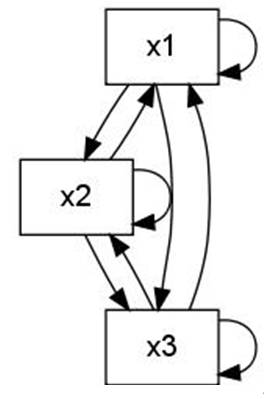
\includegraphics[scale=0.55]{exampleWD.jpg}
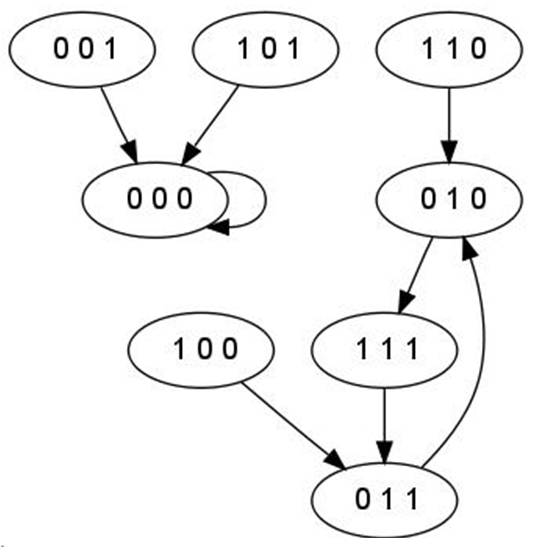
\includegraphics[scale=0.55]{exampleSS.jpg}
\caption{(left)
Wiring diagram: static relationship between variables
(right)
Phase space: temporal evolution of the system
}
\label{fig:ex}
\end{figure}
\subsubsection{Probabilistic Polynomial Dynamical System}
A {\bf probabilistic PDS} over a finite field $k$ is a collection of functions
$$f = (\{f_{1,1}, \ldots, f_{1, r_1}\}, \ldots, \{f_{n, 1}, \ldots, f_{n, r_n}
\}) : k^n \rightarrow k^n,$$
together with a probability distribution for every coordinate that assigns the
probability that a specific function is chosen to update that coordinate.
The coordinate functions $f_{i,j}$ are in $k[x_1, \ldots , x_n]$.
Probabilistic PDS, specifically Boolean probabilistic networks (PBN), have been studied
extensively in \cite{shmulevich}.
ADAM analyzes probabilistic PDS. It can simulate the
complete phase space for small enough models, by generating every possible
transition and labeling the edge with its probability according to the
distribution. If no distribution is given, ADAM assumes a uniform distribution
on all functions. For large networks, ADAM's {\it Algorithm} choice computes
steady states of probabilistic networks.
%%%%%%%%%%%
\subsubsection{Functional Edges} \label{sec:func}
An edge in the wiring diagram from $x_i$ to $x_j$ is considered
functional, if there exists a state $\hat x = (\hat x_1,  \ldots, \hat x_n)$ such
that $f_j( \hat x_1,  \ldots, a, \ldots \hat x_n) \neq f_j(\hat x_1, \ldots, b, \ldots
\hat x_n)$, where $a$ and $b$ are values for $x_i$, in other words, if there
is at least one state, such that changing only $x_i$ but keeping all other
values fixed, changes the next state of $x_j$.
In ADAM, all edges in the wiring diagram are functional.
For Boolean networks, ADAM identifies all functional circuits. A circuit is a
closed directed path in the wiring diagram and it is functional, if all its
edges are functional. For further discussion of
functional circuits, see \cite{Chaouiya}.
%%%%%%%%%%%%%%%%%%%%%%%%%%%%%%%%%%%%%%%%%%%%%%%%%%%%%%%%%%%%%%%%%%
\section{Algorithms}
\subsection{Analysis of stable attractors}
Every attractor in a PDS is either a
steady state or a limit cycle. For small models, ADAM determines the complete
phase space by enumeration, for large models, ADAM computes steady states and
limit cycles of a given length.
A state is a steady state, if it transitions to itself after one update of the
system. A state is part of a limit cycle of length $m$, if,
after $m$ updates, it results in itself. Any steady state of a PDS satisfies
the equation $f(x) = x$, as no coordinate of $x$ is changing as it is updated.
Similarly, states of a
limit cycle of length $m$ satisfy the equation $f^m(x) = x$. ADAM computes all
steady states by solving the system $f_i(x) - x_i = 0$ for $i \in \{1, \ldots,
n\}$ simultaneously. To efficiently solve the resulting systems of polynomial
equations, we first compute the Gr\"obner
basis in lexicographic order for the ideal generated by the equations.
By the elimination and extension theorem \cite{IVA}, choosing a lexicographic order
allows to easily obtain the solutions.
We use the Gr\"obner basis calculations distributed with Macaulay2 \cite{M2}, a
computer algebra system, and found that for quotient rings over a finite field
the implementation `Sugarless' is more efficient than the default algorithm
with `Sugar' \cite{Sugar:1991}.
For limit cycles of length $m$, the solutions of $f^m(x)=x$ are found and then
grouped into cycles, by applying $f$ to each of the solutions.
%%%%%%%%%%%
\subsection{Conjunctive/Disjunctive Networks} \label{sec:conj}
Some classes of networks have a certain structure that can be
exploited to achieve faster calculations. In \cite{conjunctive}, Jarrah et al.
show that for conjunctive (disjunctive) networks key dynamic features can be found with
almost no computational effort. Conjunctive (resp disjunctive) networks consist of
functions using only the AND (resp. OR) operator.
We include a separate algorithm to analyze
dynamics in the case of conjunctive/disjunctive networks as described in
\cite{conjunctive}. Currently,
this option is only implemented for networks with strongly connected dependency graphs
%%%%%%%%%%%%%%%%%%%%%%%%%%%%%%%%%%%%%%%%%%%%%%%%%%%%%%%%%%%%%%%%%%
\section*{Acknowledgments}
The authors would like to thank Claudine Chaouyia and Monika Heiner for helpful discussions. E. Dimitrova, Clemson University; J. Adeyeye, Winston-Salem State University; B. Stigler, Southern Methodist University; R. Isokpehi, Jackson State University are currently expanding ADAM’s Model Repository.
Funding for this work was provided through U.S. Army Research Office Grant Nr. W911NF-09-1-0538,
National Science Foundation Grant Nr. CMMI-0908201, and National Science Foundation Grant Nr. 0755322.


\bibliographystyle{plain}
%\bibliographystyle{authordate1}
\bibliography{ADAM}
\end{document}

